\documentclass{article}

\usepackage{tikz}
\usepackage{pgfplots}
\usepackage{verbatim}

\usepackage[top=1in, bottom=1.5in, left=1in, right=1in]{geometry}

\usepackage{graphicx}

\author{Wei Dai (CSIL: wdai, PERM: 6925747), Stefan Seritan (PERM: 5466644)}
\date{\today}
\title{CS140 Final Project Proposal:\\A Parallel Metropolis Monte Carlo Simulation}

\begin{document}
\maketitle

\section*{Background}
Simulations are a powerful tool to test and explore different chemical and physical models. In chemistry, two main types of simulations are utilized: Molecular Dynamics (MD) and Monte Carlo (MC). In MD simulations, an initial state is propagated through time to a final state using classical physics. The galactic evolution project (Homework 3) was an example of an MD-type simulation. Unlike MD simulations, Monte Carlo simulations are governed by statistical mechanics, not classical mechanics. As a result, MC simulations can perform unphysical moves, reaching equilibrium quickly (but losing any dynamic information). The principle of ergodicity states that the results of an MD and MC simulation will be the same if they are run for a sufficient time (i.e. time averages are equivalent to space averages); therefore, Monte Carlo simulations are perfect for calculating equilibrium properties quickly.\\
Furthermore, parallelizing Monte Carlo simulations is much more tractable than parallelizing MD simulations. Since MD simulations are evolved through time, processors would need be synchronized for every time step, requiring a lot of communication (as we saw in Homework 3). MC simulations, on the other hand, have no concept of time, and therefore moves only need to be spatially localized. This is still a non-trivial problem; in fact, this is an active area of research in computational chemistry. 

\section*{Simulation Details}
We will be representing the system as a Potts Lattice Gas (PLG) model. Essentially, the PLG model means that particles are set on a 3D lattice and they have two attributes: identity and orientation. We are modeling a binary mixture of particles; therefore, the identity attribute is either 1 or 2, representing the species of the particle. Orientation is an integer between 1 and 6, and represents which way the particle is "pointing" (up, down, left, right, front, or back). The data is stored as two 3-dimensional arrays. A graphical representation of our model is shown in Figure 1 below.

\begin{center}
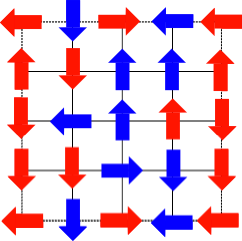
\includegraphics[scale=0.6]{PLG.png}\\
\textbf{Figure 1.} A graphical representation of the PLG model.
\end{center}

\newpage

We will be using the Metropolis formulation of the Monte Carlo simulation in a canonical (constant-$NVT$) ensemble. A Metropolis Monte Carlo simulation has the following procedure:
\begin{itemize}
\item Pick a random move
\item Calculate the change in energy ($\Delta E$) associated with the random move
\item Calculate the Boltzmann probability $p = \min\left\{1, e^{-\Delta E/k_B T}\right\}$, where $k_B$ is the Boltzmann constant and $T$ is temperature
\item Calculate a random number $r \in [0,1]$
\item Accept the move if $p > r$, reject the move if $p \leq r$
\end{itemize}
In the canonical ensemble, the number of particles ($N$), volume ($V$), and temperature ($T$) are fixed. There are two types of allowed moves. The first is a rotation, where a random particle's orientation is changed. The second is a particle swap, where two particles in random locations are exchanged. The type of move is also chosen randomly, and the two moves have equal probability of occurring.\\
The final simulation detail is the choice of Hamiltonian (i.e. how we calculate the energy of the system). For simplicity, we will use the following Hamiltonian:
$$H_0 = - \sum_{<i,j>}^{\textrm{all pairs}} \delta_{m(i),m(j)} K + \delta_{s(i),s(j)} A$$
where $m(i)$ and $s(i)$ are the identity and orientation of particle $i$. In plain English, if two neighboring particles have the same identity, they get a favorable energy bonus. Likewise, if two neighboring particles have the same orientation, they also get an energy bonus. This Hamiltonian is too simple to have any chemical application, but it makes a good test system for the efficiency of the algorithm.

\section*{Proposed Parallelization Methods}
There are two main strategies we could use to parallelize the simulation. Firstly, the simulation can be divided geometrically, with each processor performing moves on one block of the lattice. This methodology would allow the use of MPI and could be used across a large distributed system. The major complication to this approach is that the particle swap move will require communication between processors. The communication volume would get even worse as more processors are added, so this approach will likely be unscalable.\\
The second approach is to have a master thread that generates moves and worker threads that would be responsible for actually carrying out moves. If the system size is sufficiently large, we could generate a fairly large number of moves that would not be conflicting (i.e. touch the same lattice locations). These moves could then be executed in parallel because they are completely independent of each other; the only criteria for acceptance is energy change, and energy change is only based on nearest-neighbor interactions. Given the unfeasibility of the geometric approach, we will use the global scheduler approach to generate sets of moves that multiple processors can work on independently.

\end{document}
